\documentclass[conference]{IEEEtran}
\IEEEoverridecommandlockouts

\usepackage{cite}
\usepackage{amsmath,amssymb,amsfonts}
\usepackage{algorithmic}
\usepackage{graphicx}
\usepackage{textcomp}
\usepackage{xcolor}
\def\BibTeX{{\rm B\kern-.05em{\sc i\kern-.025em b}\kern-.08em
    T\kern-.1667em\lower.7ex\hbox{E}\kern-.125emX}}


\usepackage[utf8]{inputenc}
% Auskommentieren sofern Deutsch
\usepackage[ngerman]{babel}
\usepackage{pgfplots}
\usepackage{url}

\usepackage{subcaption}
\usepackage[hidelinks]{hyperref}

\usepackage{pgfplots}
\pgfplotsset{compat=1.17}

\usepackage{tikz}
\usetikzlibrary{positioning,fit,shapes.geometric,backgrounds}

\begin{document}

\section{Anhang}

% ENTWEDER alle Ansätze mit einzelnen Plots visualisieren (2 x 3 er Figures)
% ODER:
%   Eine 3 x 3 er Figures für Fartvisualisierung 
%   und eine  3 x 3 er Figure für Fehler/Varianzen


% ------------------------- Ergebnisse: RICHTUNG -------------------------


% 3er-Figure Fahrtvisualisierung: Constant Velocity RICHTUNG 1) basic, 2) frequenz, 3) frequenz+ausfall
\begin{figure*}
    \begin{subfigure}{.333\textwidth}
        \centering
        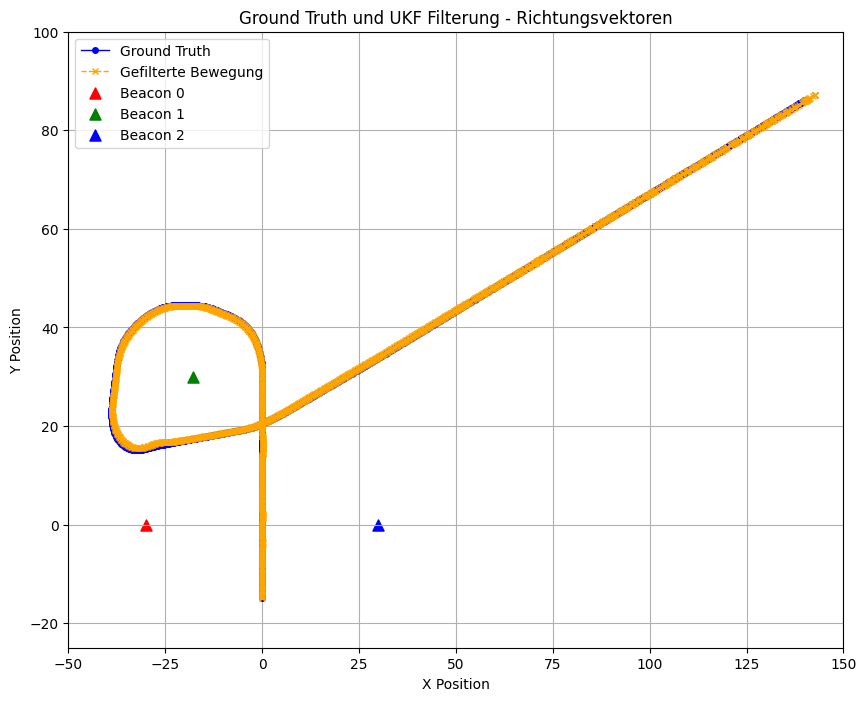
\includegraphics[width=.9\linewidth]{Ergebnisse/plots_fahrten/richtung/richtung_const_vel_basic.png}  
        \caption{Optimale Simulationsbedinungen}
        % \label{}
    \end{subfigure}    
    \begin{subfigure}{.333\textwidth}
        \centering
        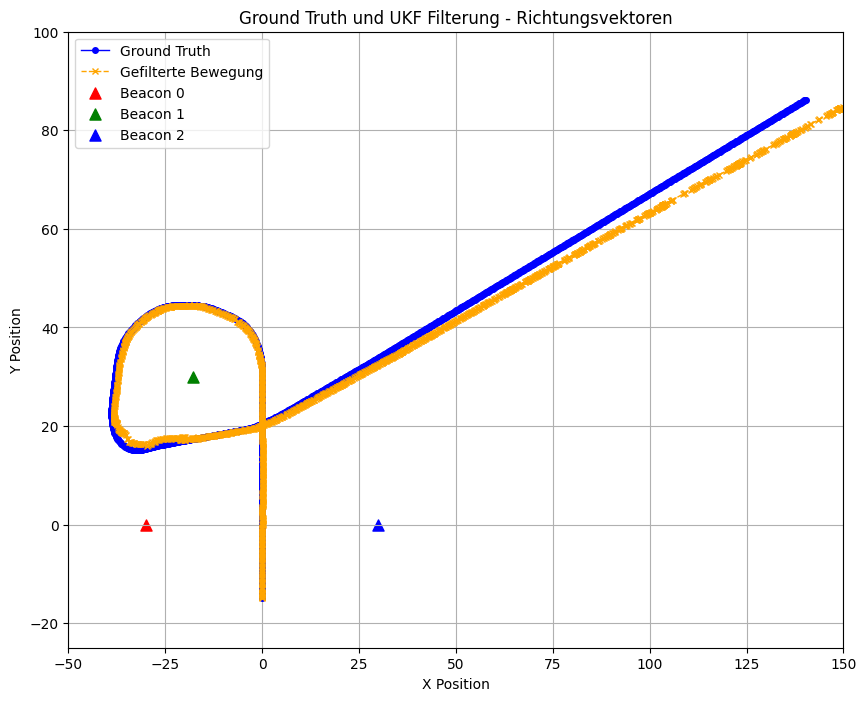
\includegraphics[width=.9\linewidth]{Ergebnisse/plots_fahrten/richtung/richtung_const_vel_freq.png} 
        \caption{Türme unterschiedlich frequent}
    \end{subfigure}    
    \begin{subfigure}{.333\textwidth}
        \centering
        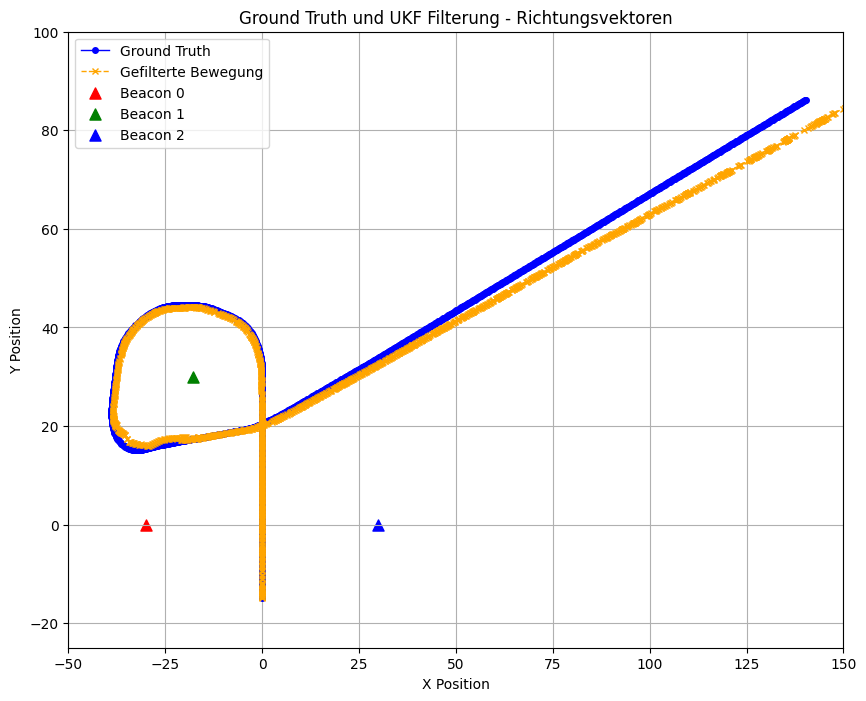
\includegraphics[width=.9\linewidth]{Ergebnisse/plots_fahrten/richtung/richtung_const_vel_flag_freq.png}
        \caption{Türme unterschiedlich frequent, ausfallend}
    \end{subfigure}
    \caption{Richtungsansatz: Ergebnisse bei konstanter Geschwindigkeit}
\end{figure*}


% 3er-Figure Fehler/Varianzen: Constant Velocity RICHTUNG 1) basic, 2) frequenz, 3) frequenz+ausfall
\begin{figure*}
    \begin{subfigure}{.333\textwidth}
        \centering
        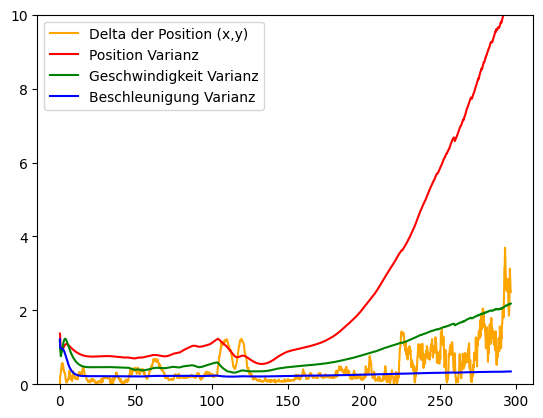
\includegraphics[width=.9\linewidth]{Ergebnisse/plots_ungenauigkeiten/richtung/richtung_const_vel_basic.png}
        \caption{Optimale Simulationsbedinungen}
    \end{subfigure}    
    \begin{subfigure}{.333\textwidth}
        \centering
        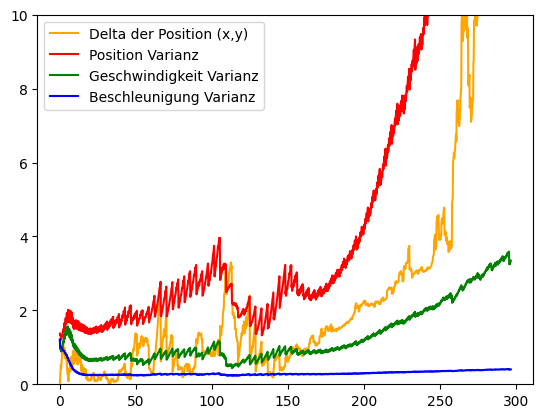
\includegraphics[width=.9\linewidth]{Ergebnisse/plots_ungenauigkeiten/richtung/richtung_const_vel_freq.png}
        \caption{Türme unterschiedlich frequent}
    \end{subfigure}    
    \begin{subfigure}{.333\textwidth}
        \centering
        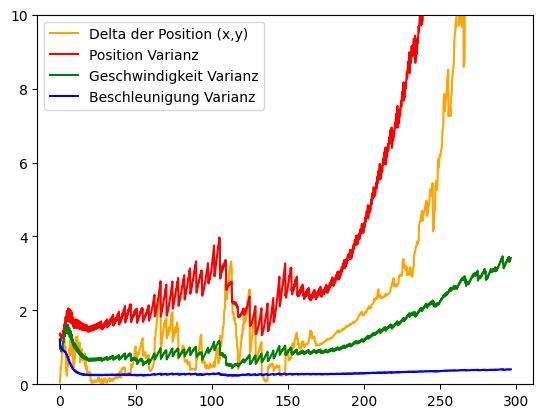
\includegraphics[width=.9\linewidth]{Ergebnisse/plots_ungenauigkeiten/richtung/richtung_const_vel_flag_freq.png}
        \caption{Türme unterschiedlich frequent, ausfallend}
    \end{subfigure}
    \caption{Richtungsansatz: Fehler und Varianzen bei konstanter Geschwindigkeit}
    \label{abb:richtung-cv-fehler}
\end{figure*}




% % ------------------------- Ergebnisse: ENTFERNUNG -------------------------

% \subsubsection{Entfernungsansatz}

% 3er-Figure Fahrtvisualisierung: Constant Velocity ENTFERNUNG 1) basic, 2) frequenz, 3) frequenz+ausfall
\begin{figure*}
    \begin{subfigure}{.333\textwidth}
        \centering
        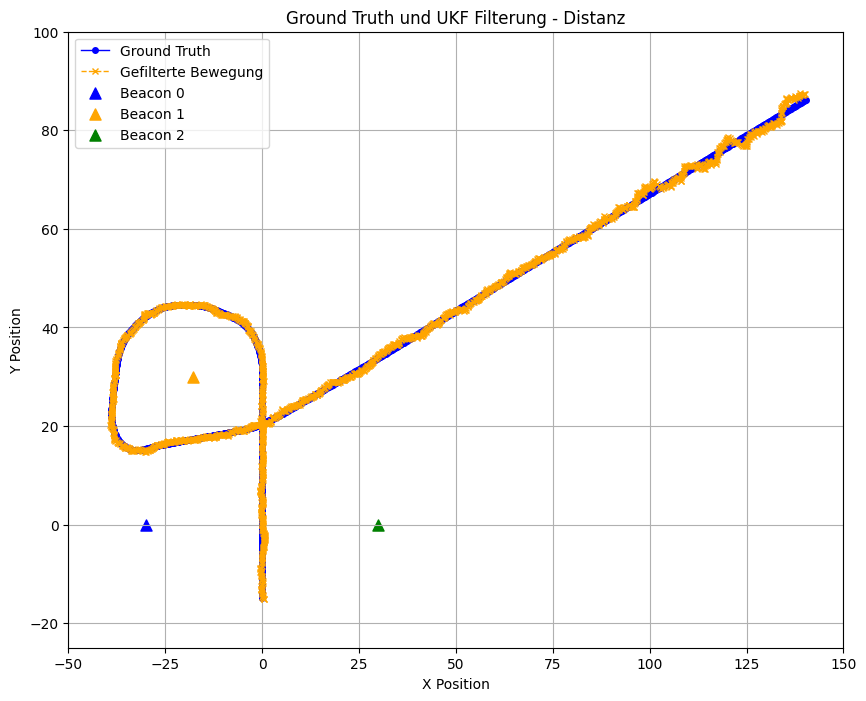
\includegraphics[width=.9\linewidth]{Ergebnisse/plots_fahrten/distanz/distanz_const_vel_basic.png}  
        \caption{Optimale Simulationsbedinungen}
    \end{subfigure}    
    \begin{subfigure}{.333\textwidth}
        \centering
        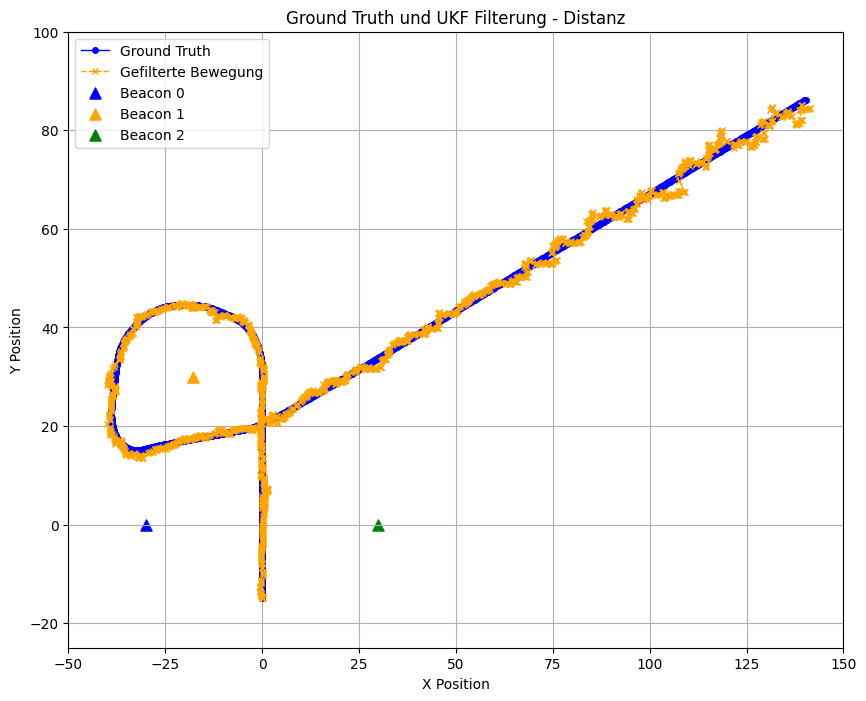
\includegraphics[width=.9\linewidth]{Ergebnisse/plots_fahrten/distanz/distanz_const_vel_freq.png} 
        \caption{Türme unterschiedlich frequent}
    \end{subfigure}    
    \begin{subfigure}{.333\textwidth}
        \centering
        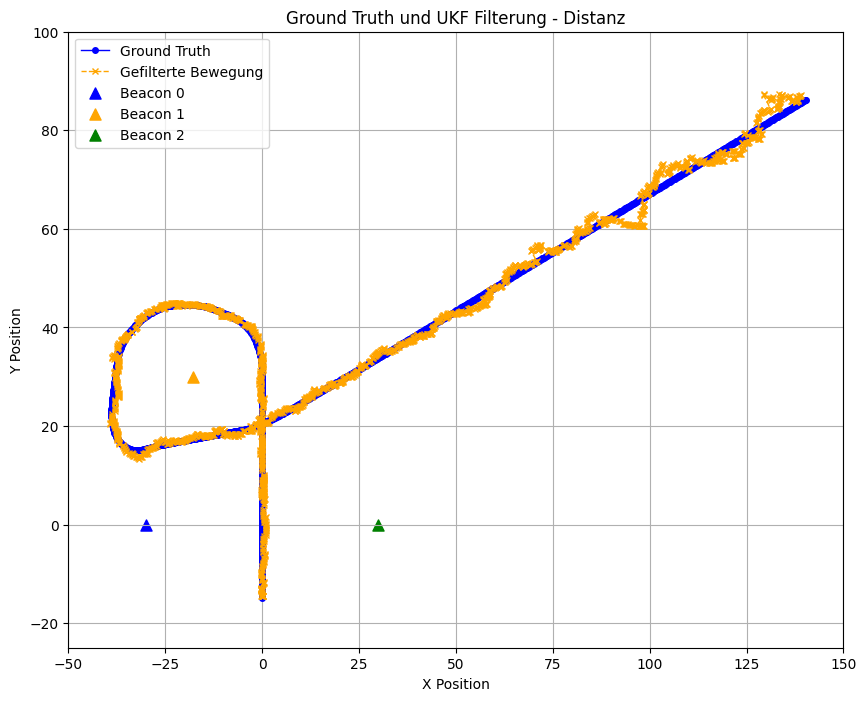
\includegraphics[width=.9\linewidth]{Ergebnisse/plots_fahrten/distanz/distanz_const_vel_flag_freq.png}
        \caption{Türme unterschiedlich frequent, ausfallend}
    \end{subfigure}
    \caption{Entfernungsansatz: Ergebnisse bei konstanter Geschwindigkeit}
\end{figure*}


% 3er-Figure Fahrtvisualisierung: Constant Velocity ENTFERNUNG 1) basic, 2) frequenz, 3) frequenz+ausfall
\begin{figure*}
    \begin{subfigure}{.333\textwidth}
        \centering
        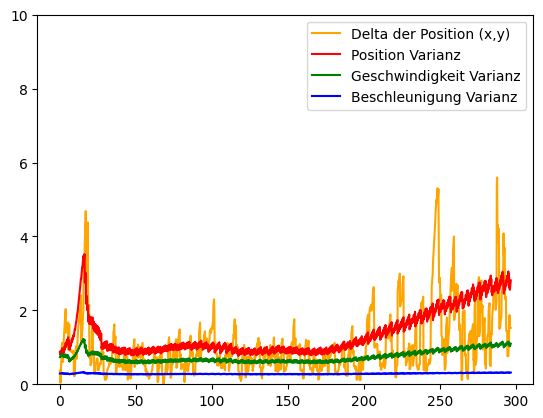
\includegraphics[width=.9\linewidth]{Ergebnisse/plots_ungenauigkeiten/distanz/distanz_const_vel_flag_freq.png}
        \caption{Optimale Simulationsbedinungen}
    \end{subfigure}    
    \begin{subfigure}{.333\textwidth}
        \centering
        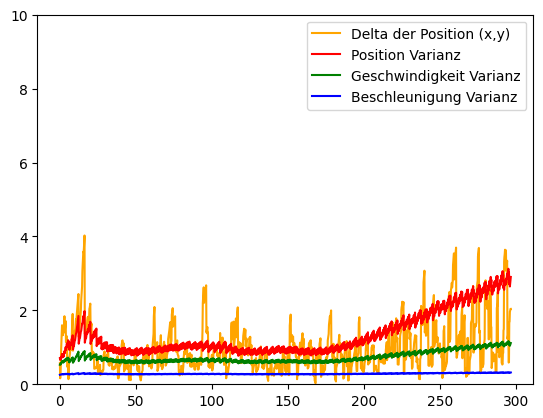
\includegraphics[width=.9\linewidth]{Ergebnisse/plots_ungenauigkeiten/distanz/distanz_const_vel_freq.png}
        \caption{Türme unterschiedlich frequent}
    \end{subfigure}    
    \begin{subfigure}{.333\textwidth}
        \centering
        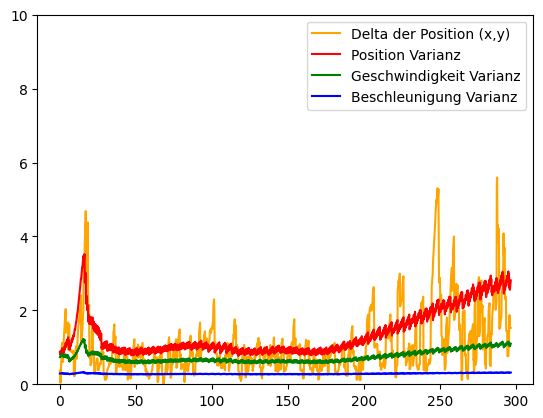
\includegraphics[width=.9\linewidth]{Ergebnisse/plots_ungenauigkeiten/distanz/distanz_const_vel_flag_freq.png}
        \caption{Türme unterschiedlich frequent, ausfallend}
    \end{subfigure}
    \label{abb:distanz-cv-fehler}
    \caption{Entfernungsansatz: Fehler und Varianzen bei konstanter Geschwindigkeit}
\end{figure*}




% % ------------------------- Ergebnisse: WINKEL -------------------------

% \subsubsection{Winkelansatz}

% 3er-Figure Fahrtvisualisierung: Constant Velocity WINKEL 1) basic, 2) frequenz, 3) frequenz+ausfall
\begin{figure*}
    \begin{subfigure}{.333\textwidth}
        \centering
        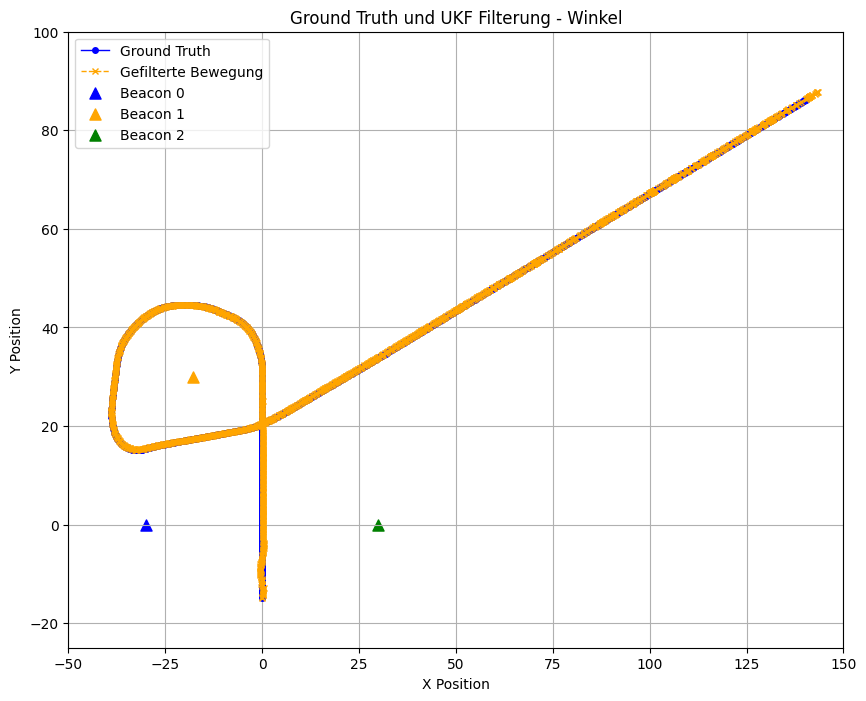
\includegraphics[width=.9\linewidth]{Ergebnisse/plots_fahrten/winkel/winkel_const_vel_basic.png}  
        \caption{Optimale Simulationsbedinungen}
        % \label{}
    \end{subfigure}    
    \begin{subfigure}{.333\textwidth}
        \centering
        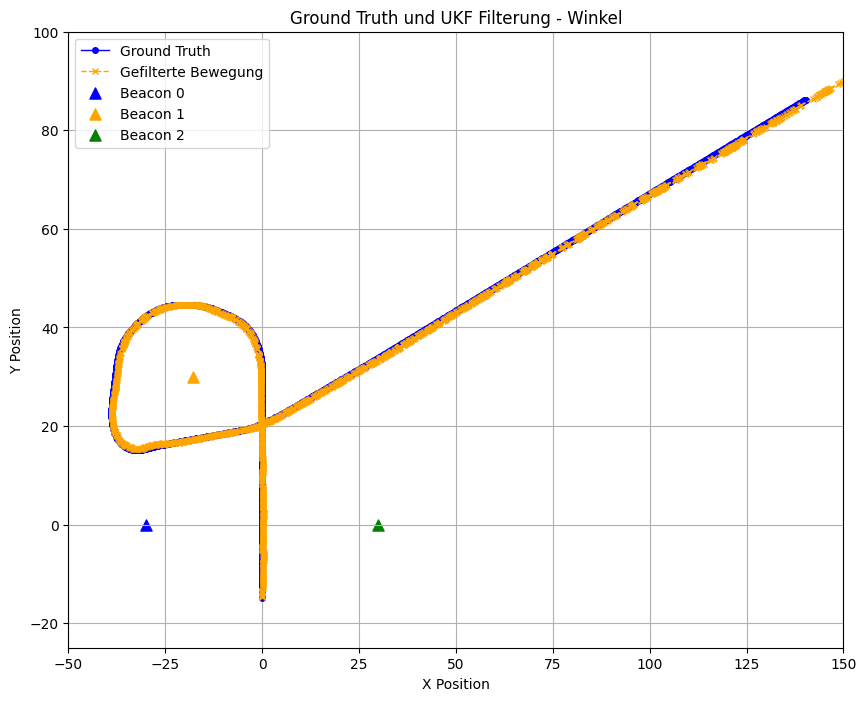
\includegraphics[width=.9\linewidth]{Ergebnisse/plots_fahrten/winkel/winkel_const_vel_freq.png} 
        \caption{Türme unterschiedlich frequent}
    \end{subfigure}    
    \begin{subfigure}{.333\textwidth}
        \centering
        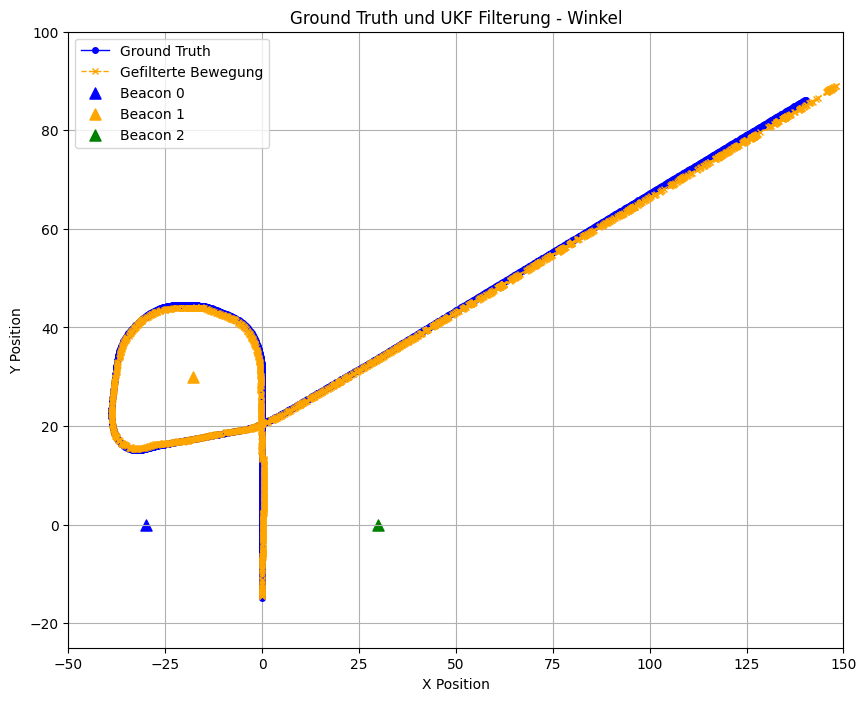
\includegraphics[width=.9\linewidth]{Ergebnisse/plots_fahrten/winkel/winkel_const_vel_flag_freq.png}
        \caption{Türme unterschiedlich frequent, ausfallend}
    \end{subfigure}
    \caption{Winkelansatz: Ergebnisse bei konstanter Geschwindigkeit}
\end{figure*}

% 3er-Figure Fehler/Varianzen: Constant Velocity WINKEL 1) basic, 2) frequenz, 3) frequenz+ausfall
\begin{figure*}
    \begin{subfigure}{.333\textwidth}
        \centering
        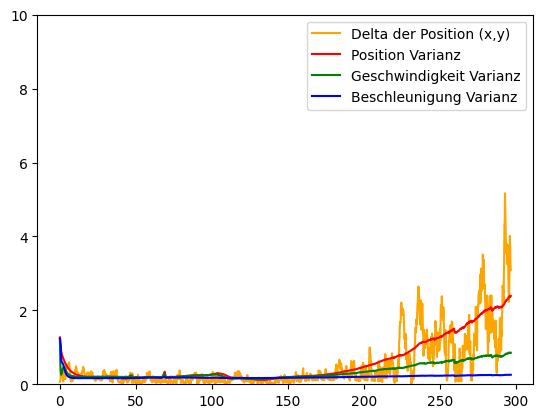
\includegraphics[width=.9\linewidth]{Ergebnisse/plots_ungenauigkeiten/winkel/winkel_const_vel_basic.png}  
        \caption{Optimale Simulationsbedinungen}
        % \label{}
    \end{subfigure}    
    \begin{subfigure}{.333\textwidth}
        \centering
        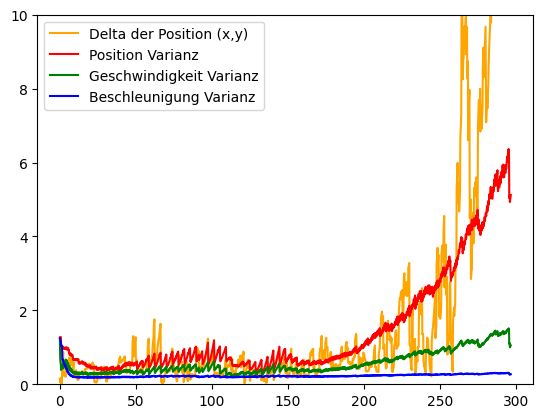
\includegraphics[width=.9\linewidth]{Ergebnisse/plots_ungenauigkeiten/winkel/winkel_const_vel_freq.png}  
        \caption{Türme unterschiedlich frequent}
    \end{subfigure}    
    \begin{subfigure}{.333\textwidth}
        \centering
        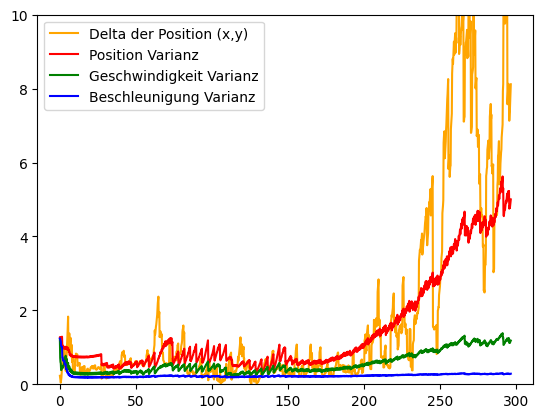
\includegraphics[width=.9\linewidth]{Ergebnisse/plots_ungenauigkeiten/winkel/winkel_const_vel_flag_freq.png}
        \caption{Türme unterschiedlich frequent, ausfallend}
    \end{subfigure}
    \caption{Winkelansatz: Fehler und Varianzen bei konstanter Geschwindigkeit}
    \label{abb:winkel-cv-fehler}
\end{figure*}



% im Vergleich lässt sich sagen, dass ... unter den in Figur ... dargestellten Filtereinstellungen am besten abschneidet.
% Wird Q optimal gesetzt, kann ... einen RMSE von bis zu ... erreichen. (Entweder besser oder schlechter als was auch immer unter nicht-Q-optimierten Bedingungen "gewonnen" hat)

% \subsection{Dynamische Geschwindigkeit}

%  ------------------------- Ergebnisse: RICHTUNG -------------------------

% \subsubsection{Richtungsansatz}

% 3er-Figure Fahrtvisualisierung: Dynamic Acceleration RICHTUNG 1) basic, 2) frequenz, 3) frequenz+ausfall
\begin{figure*}
    \begin{subfigure}{.333\textwidth}
        \centering
        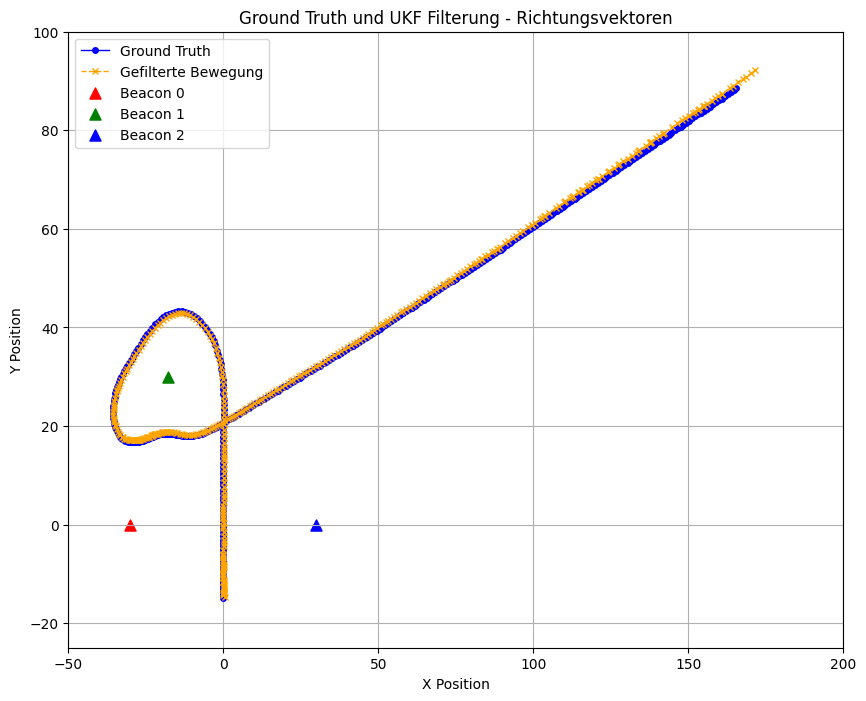
\includegraphics[width=.9\linewidth]{Ergebnisse/plots_fahrten/richtung/richtung_dyn_acc_basic.png}  
        \caption{Optimale Simulationsbedinungen}
        % \label{}
    \end{subfigure}    
    \begin{subfigure}{.333\textwidth}
        \centering
        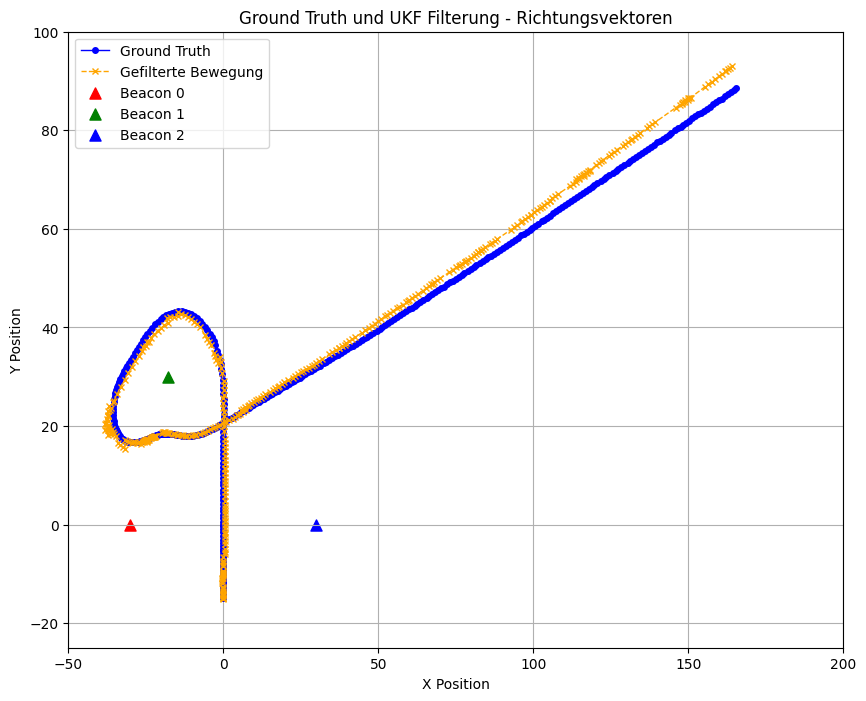
\includegraphics[width=.9\linewidth]{Ergebnisse/plots_fahrten/richtung/richtung_dyn_acc_freq.png} 
        \caption{Türme unterschiedlich frequent}
    \end{subfigure}    
    \begin{subfigure}{.333\textwidth}
        \centering
        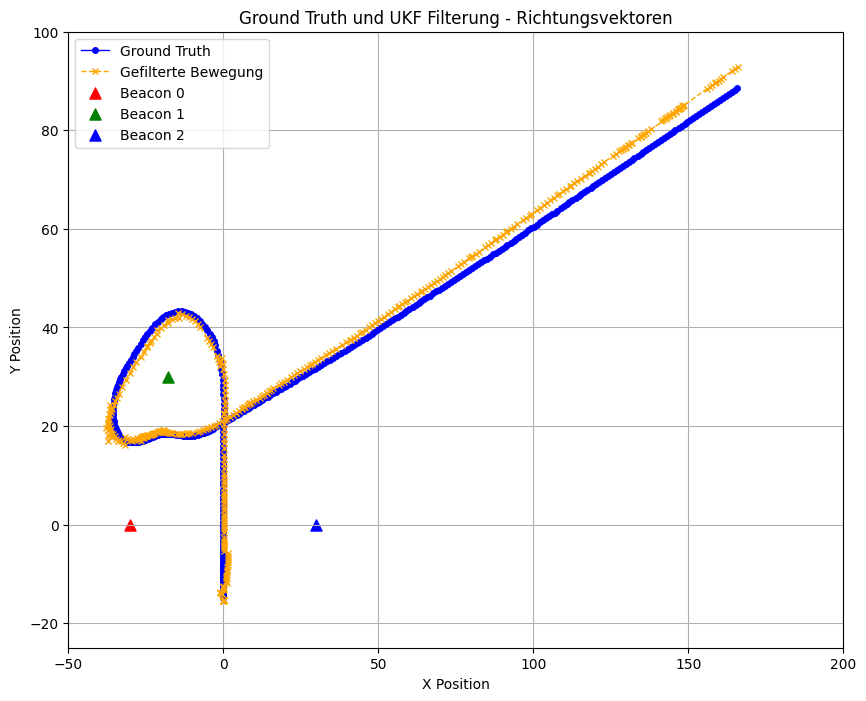
\includegraphics[width=.9\linewidth]{Ergebnisse/plots_fahrten/richtung/richtung_dyn_acc_flag_freq.png}
        \caption{Türme unterschiedlich frequent, ausfallend}
    \end{subfigure}
    \caption{Richtungsansatz: Ergebnisse bei konstanter Geschwindigkeit}
\end{figure*}

% 3er-Figure Fehler/Varianzen: Dynamic Acceleration RICHTUNG 1) basic, 2) frequenz, 3) frequenz+ausfall
\begin{figure*}
    \begin{subfigure}{.333\textwidth}
        \centering
        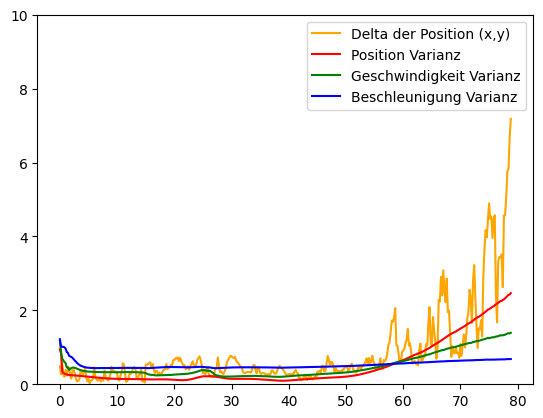
\includegraphics[width=.9\linewidth]{Ergebnisse/plots_ungenauigkeiten/richtung/richtung_dyn_acc_basic.png}
        \caption{Optimale Simulationsbedinungen}
    \end{subfigure}    
    \begin{subfigure}{.333\textwidth}
        \centering
        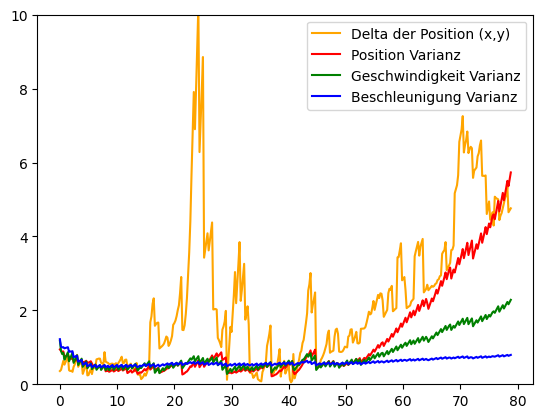
\includegraphics[width=.9\linewidth]{Ergebnisse/plots_ungenauigkeiten/richtung/richtung_dyn_acc_freq.png}
        \caption{Türme unterschiedlich frequent}
    \end{subfigure}    
    \begin{subfigure}{.333\textwidth}
        \centering
        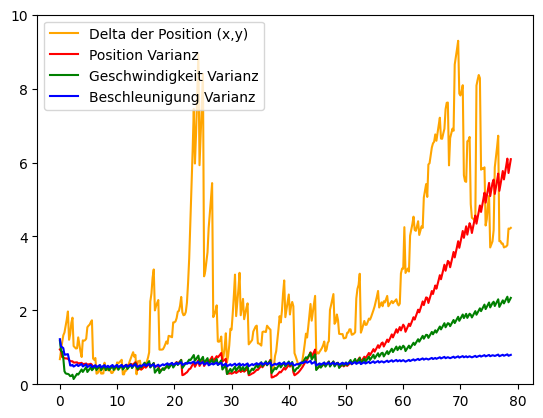
\includegraphics[width=.9\linewidth]{Ergebnisse/plots_ungenauigkeiten/richtung/richtung_dyn_acc_flag_freq.png}
        \caption{Türme unterschiedlich frequent, ausfallend}
    \end{subfigure}
    \caption{Richtungsansatz: Fehler und Varianzen bei konstanter Geschwindigkeit}
    \label{abb:richtung-da-fehler}
\end{figure*}


% % ------------------------- Ergebnisse: ENTFERNUNG -------------------------

% \subsubsection{Entfernungsansatz}

% 3er-Figure Fahrtvisualisierung: Dynamic Acceleration ENTFERNUNG 1) basic, 2) frequenz, 3) frequenz+ausfall
\begin{figure*}
    \begin{subfigure}{.333\textwidth}
        \centering
        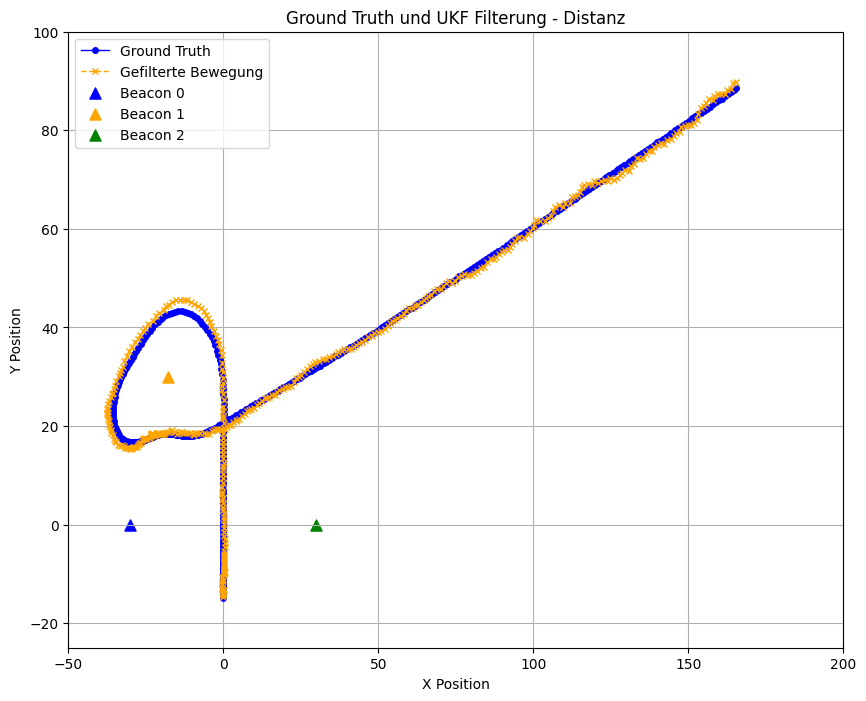
\includegraphics[width=.9\linewidth]{Ergebnisse/plots_fahrten/distanz/distanz_dyn_acc_basic.png}  
        \caption{Optimale Simulationsbedinungen}
    \end{subfigure}    
    \begin{subfigure}{.333\textwidth}
        \centering
        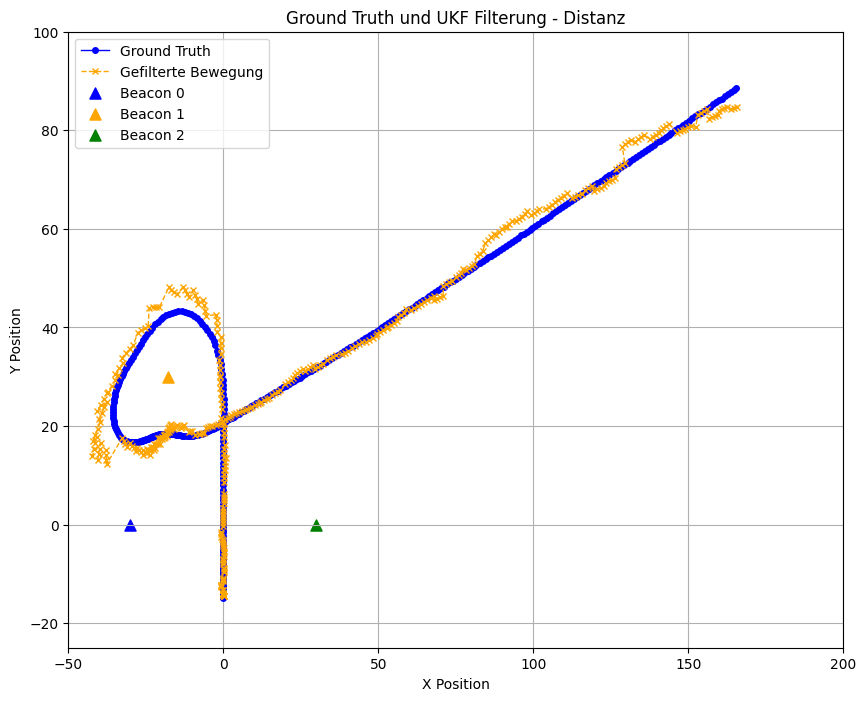
\includegraphics[width=.9\linewidth]{Ergebnisse/plots_fahrten/distanz/distanz_dyn_acc_freq.png} 
        \caption{Türme unterschiedlich frequent}
    \end{subfigure}    
    \begin{subfigure}{.333\textwidth}
        \centering
        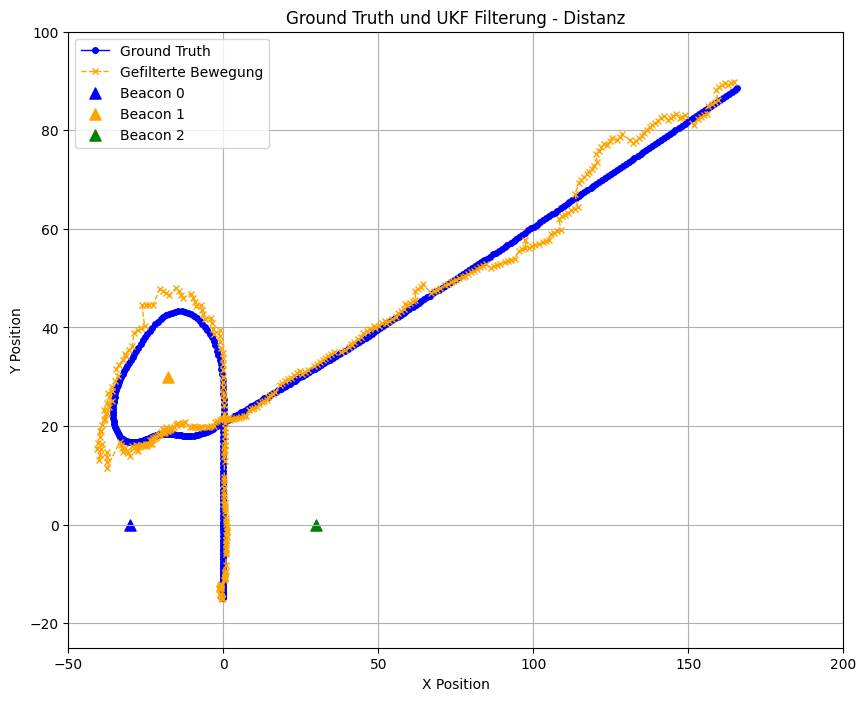
\includegraphics[width=.9\linewidth]{Ergebnisse/plots_fahrten/distanz/distanz_dyn_acc_flag_freq.png}
        \caption{Türme unterschiedlich frequent, ausfallend}
    \end{subfigure}
    \caption{Entfernungsansatz: Ergebnisse bei konstanter Geschwindigkeit}
\end{figure*}


% 3er-Figure Fahrtvisualisierung: Dynamic Acceleration ENTFERNUNG 1) basic, 2) frequenz, 3) frequenz+ausfall
\begin{figure*}
    \begin{subfigure}{.333\textwidth}
        \centering
        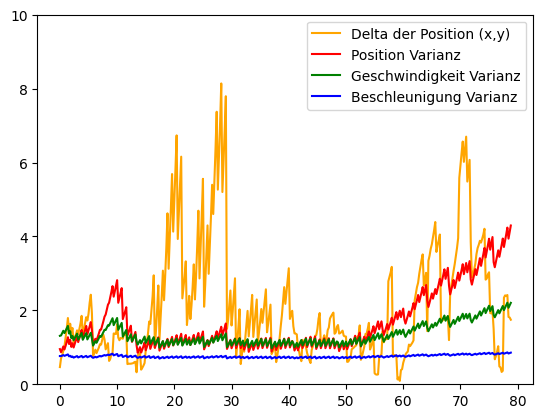
\includegraphics[width=.9\linewidth]{Ergebnisse/plots_ungenauigkeiten/distanz/distanz_dyn_acc_flag_freq.png}
        \caption{Optimale Simulationsbedinungen}
    \end{subfigure}    
    \begin{subfigure}{.333\textwidth}
        \centering
        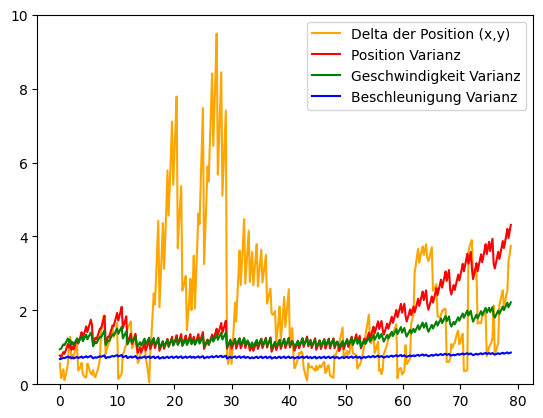
\includegraphics[width=.9\linewidth]{Ergebnisse/plots_ungenauigkeiten/distanz/distanz_dyn_acc_freq.png}
        \caption{Türme unterschiedlich frequent}
    \end{subfigure}    
    \begin{subfigure}{.333\textwidth}
        \centering
        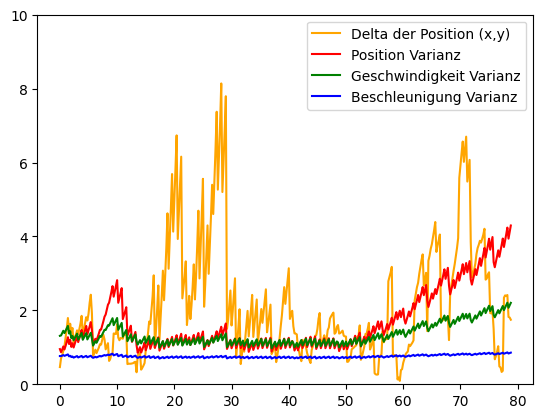
\includegraphics[width=.9\linewidth]{Ergebnisse/plots_ungenauigkeiten/distanz/distanz_dyn_acc_flag_freq.png}
        \caption{Türme unterschiedlich frequent, ausfallend}
    \end{subfigure}
    \caption{Entfernungsansatz: Fehler und Varianzen bei konstanter Geschwindigkeit}
    \label{abb:distanz-da-fehler}
\end{figure*}



% % ------------------------- Ergebnisse: WINKEL -------------------------

% \subsubsection{Winkelansatz}

% 3er-Figure Fahrtvisualisierung: Dynamic Acceleration WINKEL 1) basic, 2) frequenz, 3) frequenz+ausfall
\begin{figure*}
    \begin{subfigure}{.333\textwidth}
        \centering
        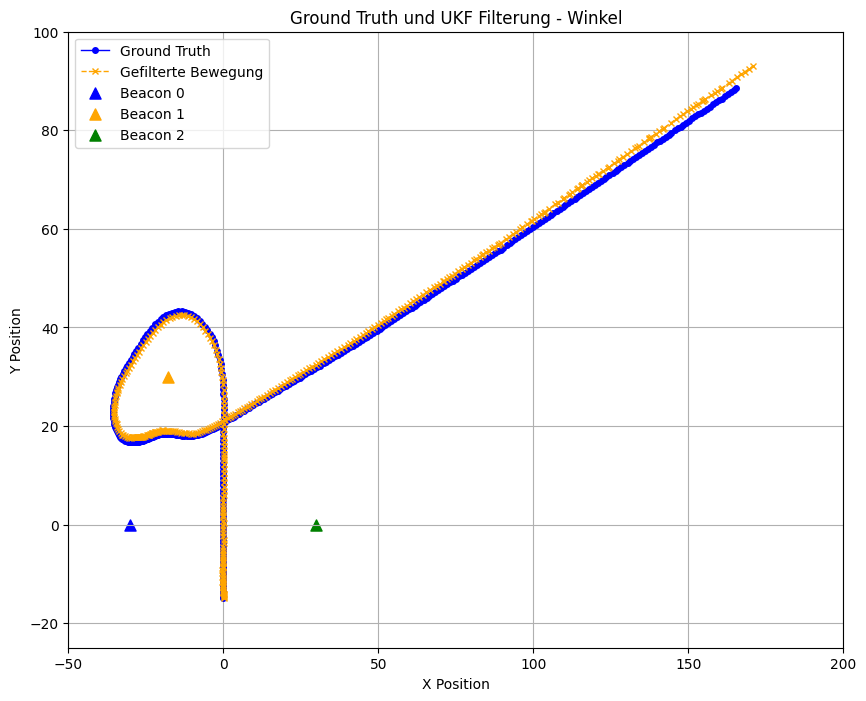
\includegraphics[width=.9\linewidth]{Ergebnisse/plots_fahrten/winkel/winkel_dyn_acc_basic.png}  
        \caption{Optimale Simulationsbedinungen}
        % \label{}
    \end{subfigure}    
    \begin{subfigure}{.333\textwidth}
        \centering
        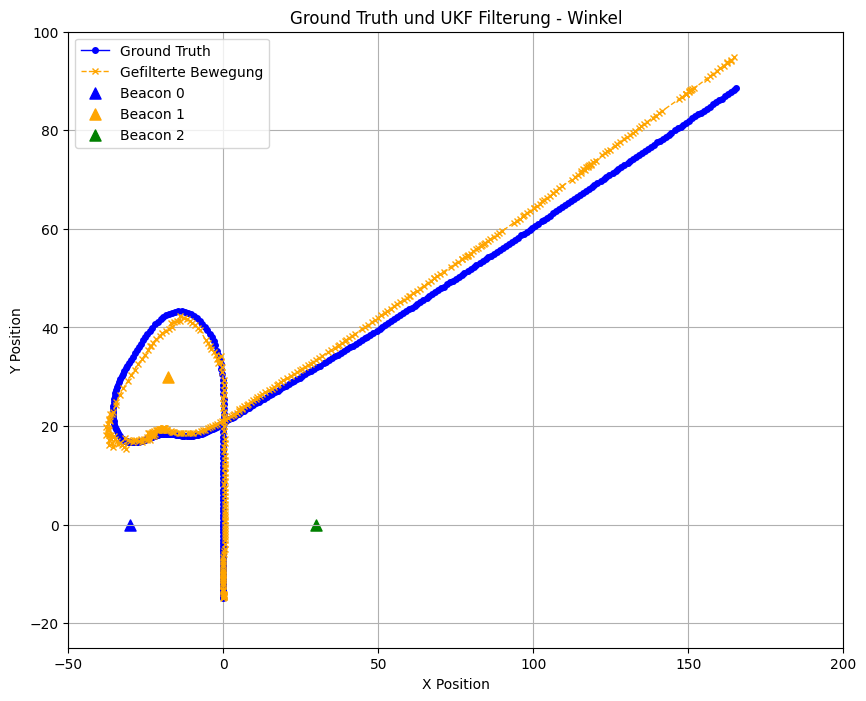
\includegraphics[width=.9\linewidth]{Ergebnisse/plots_fahrten/winkel/winkel_dyn_acc_freq.png} 
        \caption{Türme unterschiedlich frequent}
    \end{subfigure}    
    \begin{subfigure}{.333\textwidth}
        \centering
        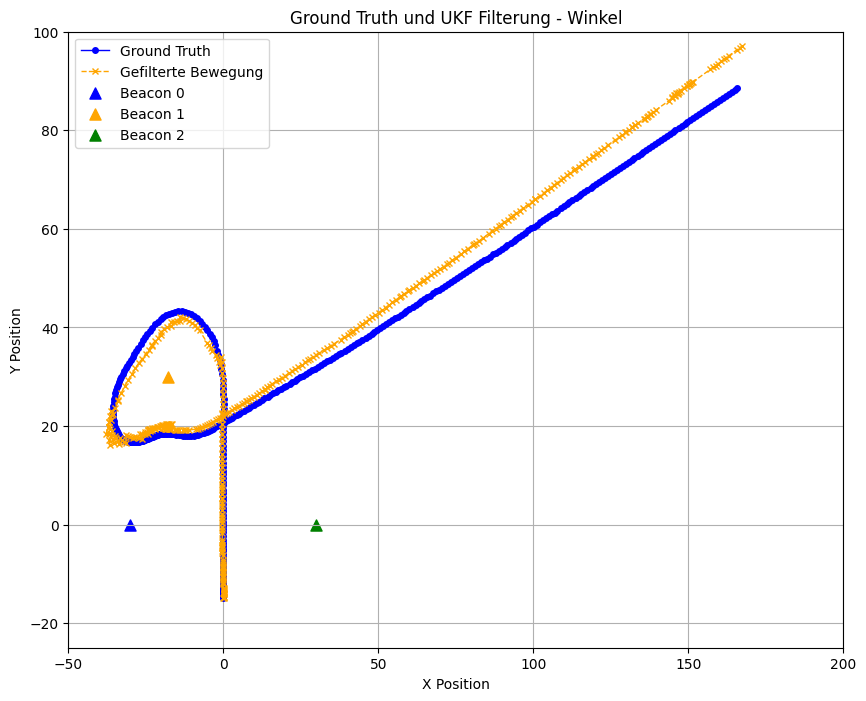
\includegraphics[width=.9\linewidth]{Ergebnisse/plots_fahrten/winkel/winkel_dyn_acc_flag_freq.png}
        \caption{Türme unterschiedlich frequent, ausfallend}
    \end{subfigure}
    \caption{Winkelansatz: Ergebnisse bei konstanter Geschwindigkeit}
\end{figure*}

% 3er-Figure Fehler/Varianzen: Dynamic Acceleration WINKEL 1) basic, 2) frequenz, 3) frequenz+ausfall
\begin{figure*}
    \begin{subfigure}{.333\textwidth}
        \centering
        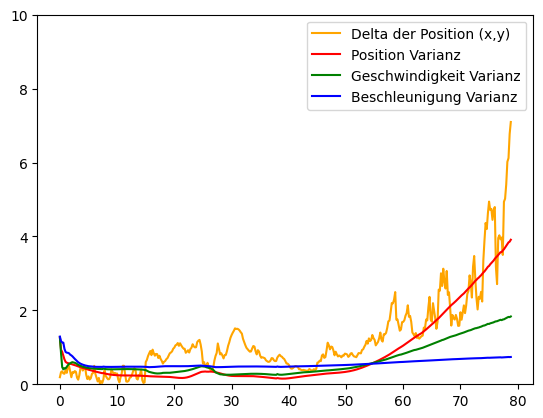
\includegraphics[width=.9\linewidth]{Ergebnisse/plots_ungenauigkeiten/winkel/winkel_dyn_acc_basic.png}  
        \caption{Optimale Simulationsbedinungen}
        % \label{}
    \end{subfigure}    
    \begin{subfigure}{.333\textwidth}
        \centering
        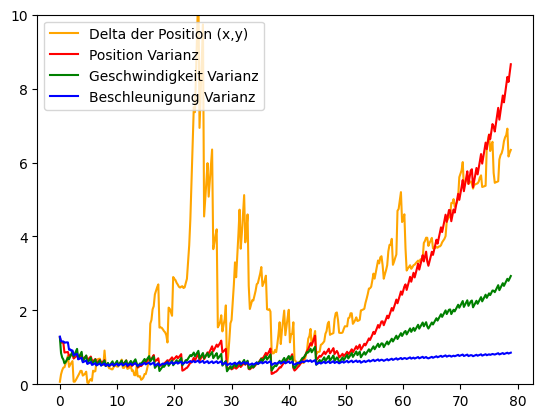
\includegraphics[width=.9\linewidth]{Ergebnisse/plots_ungenauigkeiten/winkel/winkel_dyn_acc_freq.png}  
        \caption{Türme unterschiedlich frequent}
    \end{subfigure}    
    \begin{subfigure}{.333\textwidth}
        \centering
        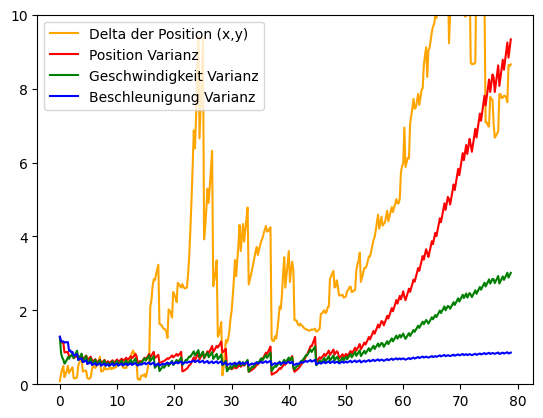
\includegraphics[width=.9\linewidth]{Ergebnisse/plots_ungenauigkeiten/winkel/winkel_dyn_acc_flag_freq.png}
        \caption{Türme unterschiedlich frequent, ausfallend}
    \end{subfigure}
    \caption{Winkelansatz: Fehler und Varianzen bei konstanter Geschwindigkeit}
    \label{abb:winkel-da-fehler}
\end{figure*}

% im Vergleich lässt sich sagen, dass ... bei optimalen Bedingungen am besten abschneidet


\end{document}